\documentclass{standalone}
\usepackage{tikz}
\usepackage{ctex,siunitx,upgreek}
\setCJKmainfont{Noto Serif CJK SC}
\usepackage{tkz-euclide}
\usepackage{amsmath}
\usetikzlibrary{patterns, calc,3d}
\usetikzlibrary {decorations.pathmorphing,decorations.pathreplacing,decorations.shapes}
\begin{document}
\small
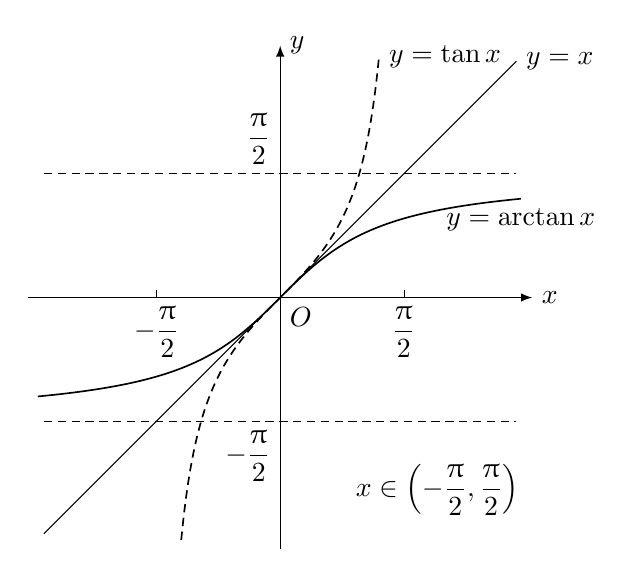
\begin{tikzpicture}[>=latex,scale=1.0]
  \draw[->](-3.2,0)--(3.2,0)node[right]{$x$};
  \draw[->](0,-3.2)--(0,3.2)node[right]{$y$};
  \node at (0,0)[below right]{$O$};
  \draw[semithick,samples=200,domain=-0.4*pi:0.4*pi] plot ({tan(\x r)},\x)node[below]{$y=\arctan x$};
  \draw[semithick,densely dashed,samples=200,domain=-0.4*pi:0.4*pi] plot (\x,{tan(\x r)})node[right]{$y=\tan x$};
  \draw(-3,-3)--(3,3)node[right]{$y=x$};
  \draw[densely dashed](-3,0.5*pi)--(3,0.5*pi);
  \draw[densely dashed](-3,-0.5*pi)--(3,-0.5*pi);
  \draw[very thin](0.5*pi,0)node[below]{$\dfrac\uppi2$}--++(0,0.1);
  \draw[very thin](-0.5*pi,0)node[below]{$-\dfrac\uppi2$}--++(0,0.1);
  \node at (0,0.5*pi)[above left]{$\dfrac\uppi2$};
  \node at (0,-0.5*pi)[below left]{$-\dfrac\uppi2$};
  \node at (2.0,-2.0)[below]{$x\in\left(-\dfrac\uppi2,\dfrac\uppi2\right)$};
\end{tikzpicture}
\end{document}